% !TeX program = xelatex
% !TeX encoding = UTF-8
% !TeX spellcheck = en_US
% !BIB program = biber
\documentclass[a4paper,oneside,10pt,english]{scrartcl}
\usepackage[techreport,nofancyfonts]{jkureport}

\usepackage{csquotes}
\usepackage[backend=bibtex,citestyle=numeric,sortcites=true,maxcitenames=2,style=ACM-Reference-Format]{biblatex}
\usepackage{array}
\usepackage{booktabs}
\usepackage{graphicx}
\usepackage{pgfplots}
\usepackage{pgfplotstable}
\usepackage{siunitx}
\usepackage{tabularx}
\usepackage{tikz}
\usepackage{xurl}

\usetikzlibrary{arrows.meta,backgrounds,calc,fit,positioning}
\usepgfplotslibrary{groupplots}
\pgfplotsset{compat=1.17}

\definecolor{ndsblue}{HTML}{255F85}
\definecolor{ndsgold}{HTML}{B57922}
\definecolor{ndsgreen}{HTML}{4E7A2E}
\definecolor{ndsred}{HTML}{A33A2B}
\definecolor{ndsgray}{HTML}{5C6670}
\newcolumntype{Y}{>{\raggedright\arraybackslash}X}

\setcounter{biburlnumpenalty}{100}
\setcounter{biburllcpenalty}{100}
\setcounter{biburlucpenalty}{100}
\addbibresource{references.bib}

\sisetup{
  detect-all,
  group-separator = {,},
  group-minimum-digits = 4,
  round-mode = places,
  round-precision = 2
}

\title{NDSwin-JAX:\texorpdfstring{\\}{ }Implementing and Evaluating an N-Dimensional\texorpdfstring{\\}{ }Shifted Window Transformer in JAX}
\titleshort{NDSwin-JAX}
\subtitle{Technical Report\texorpdfstring{\\}{ - }%
  \usekomafont{subtitlesmall}%
  Practical Work in AI (BSc)\texorpdfstring{\\}{ - }%
  \usekomafont{subtitlesmall}Institute for Machine Learning, Johannes Kepler University Linz%
}
\author{Volodymyr Yelisieiev\matno{12340334}}
\supervisor[1,male]{Gianluca Galletti}
\submissiondepartment{KUSSS IDs 365.266 / 365.267\texorpdfstring{\\}{ - }Semester: SS 2026}
\date{2026-04-30}
\revisionblock{%
Public repository:\texorpdfstring{\\}{ - }%
\url{https://github.com/volodymyr-yelisieiev/ndswin-jax}%
}

\begin{document}
\maketitle

\cleardoubleoddpage
\tableofcontents

\cleardoubleoddpage
\addsec{Abstract}
This report presents \emph{NDSwin-JAX}, a JAX/Flax implementation of the Swin Transformer that was refactored into a genuinely N-dimensional framework. The core engineering objective was to preserve the shifted-window design of the original Swin architecture while removing its hard dependency on 2D image grids. In practice, that meant rewriting patch embedding, window partitioning and reversal, cyclic shifting, relative position indexing, and hierarchical stage composition so that they operate on arbitrary spatial dimensionalities controlled only by configuration.

The final publishable artifact set evaluates the implementation on three workloads: 2D classification on CIFAR-10, 2D classification on CIFAR-100, and 3D voxel classification on a ModelNet40 export. The saved restored-best checkpoints reach validation top-1 accuracies of \(0.9182\) on CIFAR-10, \(0.6948\) on CIFAR-100, and \(0.7421\) on ModelNet40. Recomputed held-out test evaluations are also preserved for the final checkpoints, with test top-1 accuracies of \(0.8995\), \(0.6963\), and \(0.6965\), respectively.

These results support the central claim of the project: the implementation successfully generalizes shifted-window transformers beyond 2D and remains trainable on both image and voxel inputs under a shared software stack. The report stays conservative about scope. The evidence consists of single retained runs rather than repeated-seed experiments, and the 3D result uses a voxelized ModelNet40 export rather than a raw point-cloud protocol. Consequently, the contribution is best understood as a traceable implementation and empirical validation study rather than a state-of-the-art benchmark claim.


\cleardoubleoddpage
\section{Introduction}
\label{sec:introduction}
Vision transformers have changed how visual recognition models are designed, but early transformer architectures often scaled poorly with input resolution because self-attention was computed globally over all tokens. The original Swin Transformer addressed this issue by replacing global attention with a hierarchy of local windowed attention blocks and a shifted-window mechanism that lets neighboring windows exchange information without restoring full quadratic attention cost across the entire image \citep{liu2021swin}. This design made transformer-based models much more practical for mainstream computer vision tasks and established Swin as one of the most influential hierarchical transformer backbones.

The limitation that motivated this project is that most implementations and much of the surrounding tooling remain strongly biased toward 2D imagery. In many research and engineering settings, however, the data are not naturally 2D. Medical scans, voxelized CAD objects, and other spatial measurements often live in three dimensions. Video and spatio-temporal signals can require even higher-dimensional reasoning. Reusing the shifted-window idea in these settings should be possible in principle, but real codebases often encode 2D assumptions in patch extraction, window bookkeeping, relative position indexing, data loading, and training orchestration. As a result, extending a 2D Swin implementation into a general N-dimensional system is less a matter of changing a single attention layer than of making the entire modeling and experimentation stack dimension-aware.

The goal of this practical work was therefore to build an N-dimensional shifted-window transformer in JAX and to verify that the resulting implementation can be trained in a realistic, traceable workflow. The emphasis of the project is not on proposing a new transformer variant. Instead, the contribution is an implementation and systems contribution: one codebase, one configuration-driven command surface, and one training stack that can support both 2D image classification and 3D voxel classification by changing configuration rather than rewriting architecture-specific code. This project also aimed to make the surrounding workflow credible from a research-practice perspective by supporting hyperparameter sweeps, queue-based job execution, logging, checkpointing, and dataset validation before a run starts.

The repository snapshot analyzed in this report contains exactly the kind of evidence needed for such a claim. It includes preserved sweeps and restored-best retraining checkpoints for CIFAR-10, CIFAR-100, and a voxelized ModelNet40 dataset. The final checkpoints reach validation top-1 accuracies of \(0.9182\), \(0.6948\), and \(0.7421\), respectively, with recomputed held-out test top-1 accuracies of \(0.8995\), \(0.6963\), and \(0.6965\). It also includes queue, tmux, and resume logs showing how the workloads were orchestrated through the same CLI-based pipeline, including the ModelNet40 rerun after a train-derived validation split was created. These artifacts demonstrate that the project is not merely a collection of isolated modules, but a functioning experimentation framework.

This report is structured as follows. \autoref{sec:related-work} situates the implementation in the context of the original Swin paper, the JAX/Flax ecosystem, and the datasets used here. \autoref{sec:methods} explains how the architecture and training system were generalized from fixed 2D assumptions to arbitrary spatial dimensionalities. \autoref{sec:setup} documents the experimental setup, the datasets, the hardware, and the sweep procedures. \autoref{sec:results} interprets the validation-selected checkpoints and the recomputed test metrics, including the gap between sweep-best and final retraining performance for ModelNet40. Finally, \autoref{sec:limitations} summarizes the main constraints of the preserved evidence, especially the lack of repeated-seed uncertainty estimates. The report deliberately stays within those limits so that every conclusion can be traced back to the saved artifacts rather than to assumptions or reconstructed claims.


\section{Related Work}
\label{sec:related-work}
NDSwin-JAX builds directly on the Swin Transformer of \citet{liu2021swin}. Swin made vision transformers more practical by replacing global attention with local window attention and shifted windows. This retained a hierarchical feature pyramid while reducing the cost of attention on dense visual grids.

The same idea has already proved useful beyond ordinary 2D classification. Video Swin adapts shifted-window attention to video recognition by adding a temporal dimension while preserving the locality and hierarchy of the original model \citep{liu2022videoswin}. Swin3D applies a Swin-style backbone to sparse 3D scene understanding, showing why local attention and relative position information are natural tools for large 3D inputs \citep{yang2023swin3d}. These projects motivate the central engineering goal of this work: implement the spatial operators once, over tuples of dimensions, instead of maintaining separate 2D and 3D code paths.

The implementation is built in JAX and Flax, which makes this project partly a software-engineering exercise in reusable array programming rather than only a model-training exercise \citep{jaxrepo,flaxrepo}. That matters for the report's central question: the evidence has to show not only that one checkpoint achieves a useful score, but that the code path remains configurable, inspectable, and reproducible across dimensionalities.

Medical imaging is especially relevant because many datasets are naturally volumetric. UNETR reformulates 3D medical segmentation as transformer-based sequence modeling with a U-shaped decoder \citep{hatamizadeh2022unetr}. Swin UNETR then combines a hierarchical Swin encoder with medical segmentation decoders and self-supervised pre-training on large CT collections \citep{tang2022swinunetrpretrain,hatamizadeh2022swinunetr}. nnFormer is another volumetric transformer that interleaves convolution and attention for 3D segmentation \citep{zhou2021nnformer}. Together, these works show that high-dimensional transformer backbones are not just a software curiosity; they are a practical direction for volumetric data.

This report is narrower than those papers. It does not propose a new medical segmentation benchmark or claim state-of-the-art accuracy. Its contribution is an auditable JAX/Flax implementation of the shifted-window backbone that can be configured for different spatial dimensionalities, plus the training and queue machinery needed to run 2D and 3D experiments reproducibly.


\section{Methods and Implementation}
\label{sec:methods}
The central implementation task was to remove implicit 2D assumptions from the Swin pipeline while preserving the original architectural pattern. In the analyzed repository snapshot, the resulting model is exposed as \texttt{NDSwinTransformer} and configured through \texttt{num\_dims}, \texttt{patch\_size}, and \texttt{window\_size}. The model still follows the familiar Swin structure: patch embedding, multiple hierarchical transformer stages, and a classifier head. The difference is that spatial operators now work on tuples of arbitrary length instead of fixed height--width pairs.

\begin{figure}[t]
  \centering
  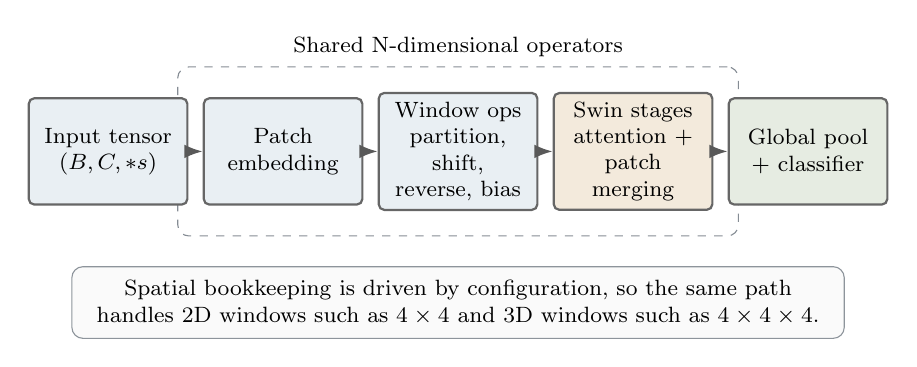
\begin{tikzpicture}[
  font=\footnotesize,
  >=Latex,
  node distance=0.18cm and 0.18cm,
  pipeline/.style={draw=black!60, rounded corners=2pt, thick, minimum height=1.35cm, text width=1.78cm, align=center},
  op/.style={pipeline, fill=ndsblue!10},
  stage/.style={pipeline, fill=ndsgold!16},
  head/.style={pipeline, fill=ndsgreen!14},
  flow/.style={-Latex, thick, draw=black!65},
  note/.style={draw=ndsgray!70, rounded corners=4pt, fill=black!2, inner sep=5pt, align=center, text width=0.78\linewidth}
]
  \node[op] (input) {Input tensor\\$(B, C, *s)$};
  \node[op, right=of input] (patch) {Patch\\embedding};
  \node[op, right=of patch] (window) {Window ops\\partition, shift,\\reverse, bias};
  \node[stage, right=of window] (stages) {Swin stages\\attention +\\patch merging};
  \node[head, right=of stages] (head) {Global pool\\+ classifier};

  \draw[flow] (input) -- (patch);
  \draw[flow] (patch) -- (window);
  \draw[flow] (window) -- (stages);
  \draw[flow] (stages) -- (head);

  \begin{scope}[on background layer]
    \node[
      draw=ndsgray!75,
      dashed,
      rounded corners=4pt,
      fit=(patch) (window) (stages),
      inner sep=9pt,
      label={[font=\footnotesize, align=center]above:Shared N-dimensional operators}
    ] {};
  \end{scope}

  \node[note, below=0.7cm of window.south] (note) {Spatial bookkeeping is driven by configuration, so the same path handles 2D windows such as \(4 \times 4\) and 3D windows such as \(4 \times 4 \times 4\).};
\end{tikzpicture}

  \caption{Overview of the N-dimensional shifted-window pipeline used in NDSwin-JAX. The grouped middle blocks are the generic spatial operators: they reuse the same code path for 2D image windows and 3D voxel windows by reading \texttt{num\_dims}, \texttt{patch\_size}, and \texttt{window\_size} from configuration.}
  \label{fig:architecture}
\end{figure}

At the model level, patch embedding converts channel-first tensors of shape \((B, C, *\text{spatial})\) into token grids whose dimensionality depends only on the configured patch size. The generalized window operators then partition tensors of shape \((B, *\text{spatial}, C)\) into local windows, reverse that partitioning after attention, and apply cyclic shifts along each spatial axis. Relative position bias indexing is likewise computed from the configured window shape. These are exactly the components that fail first in a Swin implementation that assumes only two spatial coordinates. Replacing those assumptions with tuple-based shape arithmetic lets the same attention block process both \(4 \times 4\) image windows and \(4 \times 4 \times 4\) voxel windows.

The implementation also preserves the hierarchical structure of Swin. The model stacks multiple stages, each with its own depth, number of heads, and stochastic depth schedule. Between stages, patch merging reduces spatial resolution while increasing the embedding dimension. Because these transformations operate on generic spatial tuples, the same stage logic applies to both the CIFAR-10 model and the ModelNet40 model analyzed here. In practice, moving from 2D to 3D becomes a configuration change rather than an architectural rewrite.

The project extends beyond the model definition into the training system. The repository's canonical interface is the \texttt{ndswin} CLI, which supports training, sweeps, auto-sweeps, queue execution, dataset export, and validation. This matters for reproducibility because the same command surface launches both the 2D and 3D workflows. In the preserved artifact set, a queue file schedules one auto-sweep-plus-retrain workflow for CIFAR-10 and one for ModelNet40. The evidence therefore covers both the model and the orchestration layer expected in a practical research project.

\begin{table}[t]
  \centering
  \caption{Execution environment extracted from the preserved artifact set. The software versions are grounded in \texttt{pyproject.toml}; the runtime device selection is confirmed by the saved training logs.}
  \label{tab:environment}
  \begin{tabularx}{\linewidth}{@{}lY@{}}
    \toprule
    \textbf{Item} & \textbf{Value} \\
    \midrule
    CPU & Intel Xeon E5-2630 v4, 20 logical CPUs \\
    GPU inventory & 4 \(\times\) NVIDIA GeForce GTX 1080 Ti, 11264 MiB each \\
    RAM & 125 GiB system memory \\
    Runtime device selection & 4 GPUs selected automatically for both preserved final training runs \\
    Core software & JAX 0.7.1, jaxlib 0.7.1, Flax, Optax, Orbax checkpointing \\
    \bottomrule
  \end{tabularx}
\end{table}

Training itself is implemented with JAX-based optimization and data-parallel sharding. The trainer constructs a JAX mesh over the visible devices and shards batches along the batch dimension using \texttt{NamedSharding}. This is relevant because the kept April logs show that the preserved final runs selected four GPUs automatically rather than relying on a manually fixed device list. The code chooses only devices that satisfy memory and utilization thresholds, so the report does not overstate the hardware actually used for the preserved experiments.

Finally, the implementation includes guard rails around data and configuration. Dataset contracts are validated before training starts, the ModelNet40 export is described by a manifest containing split counts and class information, and the sweep and queue layers record summaries to JSON. These details matter scientifically because they make the evidence auditable. The results reported later are extracted from structured artifacts that preserve configuration, runtime metadata, and metric histories rather than from informal notes or screenshots.


\section{Experimental Setup}
\label{sec:setup}
The experiments in this report are restricted to the final publishable artifact set preserved under \path{report/data/sources/}. This artifact set combines the repaired CIFAR-10 retraining run from May 18, 2026, the repaired CIFAR-100 sweep-and-retrain run from May 19--20, 2026, and the stabilized ModelNet40 voxel run from April 29, 2026. The goal is to document what was actually built, debugged, and measured, not to mix the strongest-looking numbers from unrelated runs.

The first workload is CIFAR-10, a 10-class image classification task with \(32 \times 32\) RGB inputs \citep{krizhevsky2009cifar}. The second workload is CIFAR-100, which keeps the same input resolution but increases the label space to 100 classes. Both CIFAR loaders use a deterministic stratified validation split from the training set and preserve the official test split for post-training evaluation. The final CIFAR-10 and CIFAR-100 checkpoints were selected by validation accuracy and then recomputed on the held-out test split.

The third workload is a voxelized ModelNet40 export \citep{wu20153dshapenets}. The repository manifest describes 8{,}858 training samples, 985 train-derived validation samples, and 2{,}468 test samples, with one input channel and a spatial resolution of \(32^3\). This experiment uses \texttt{num\_dims = 3}, which activates the generalized 3D path in patch embedding, window partitioning, shifting, and patch merging. A held-out test recomputation is preserved for the final restored checkpoint, but the report remains explicit that the model was selected by validation accuracy.

\begin{table}[t]
  \centering
  \scriptsize
  \caption{Experimental ledger for the preserved runs. Sweep budgets and summed trial wall-clock times come from the committed sweep summaries; restored epochs and final wall-clock times come from the final \texttt{metrics.json} files.}
  \label{tab:experiment-ledger}
  \begin{tabularx}{\linewidth}{@{}lYYYY@{}}
    \toprule
    \textbf{Workload} & \textbf{Splits used} & \textbf{Sweep budget/time} & \textbf{Final training state} & \textbf{Final wall-clock} \\
    \midrule
    CIFAR-10 & 45k train / 5k validation / 10k test & 48 trials, 60 epochs each; 32.83 h summed & 600-epoch budget; stopped at 392; restored epoch 352 & 14{,}866.06 s (4.13 h) \\
    CIFAR-100 & 45k train / 5k validation / 10k test & 24 trials, 50 epochs each; 13.58 h summed & 600-epoch budget; stopped at 350; restored epoch 300 & 12{,}043.98 s (3.35 h) \\
    ModelNet40 & 8{,}858 train / 985 validation / 2{,}468 test & 15 trials, 10 epochs each; 1.08 h summed & 200-epoch budget; stopped at 27; restored epoch 7 & 990.99 s (0.28 h) \\
    \bottomrule
  \end{tabularx}
\end{table}

\begin{table}[t]
  \centering
  \scriptsize
  \caption{Final retraining configurations. The table keeps the main effective knobs visible while the exact JSON and metric files remain preserved in \autoref{app:artifacts}.}
  \label{tab:retrain-configs}
  \begin{tabularx}{\linewidth}{@{}lYYY@{}}
    \toprule
    \textbf{Workload} & \textbf{Geometry and model} & \textbf{Optimization} & \textbf{Regularization} \\
    \midrule
    CIFAR-10 & 2D; patch \(2 \times 2\); window \(4 \times 4\); embed 96; depths \([2,2,18,2]\) & batch 128; lr \(4.300210 \times 10^{-4}\); wd \(1.041082 \times 10^{-2}\); warmup 20 & drop 0.05; drop path 0.1; cutmix 0.5; color jitter \\
    CIFAR-100 & 2D; patch \(2 \times 2\); window \(4 \times 4\); embed 96; depths \([2,2,18,2]\) & batch 128; lr \(2.047168 \times 10^{-4}\); wd \(2.672492 \times 10^{-2}\); warmup 30 & drop path 0.3; mixup 0.2; cutmix 0.5; cutout 16 \\
    ModelNet40 & 3D; patch \(2 \times 2 \times 2\); window \(4 \times 4 \times 4\); embed 72; depths \([2,2,6,2]\) & batch 64; lr \(1.262274 \times 10^{-3}\); wd \(7.049835 \times 10^{-3}\); warmup 3 & drop path 0.1 \\
    \bottomrule
  \end{tabularx}
\end{table}

Hyperparameter search is performed through configuration-driven random search. The preserved CIFAR-10 sweep evaluated 48 trials with validation accuracy as the selection metric and a 60-epoch budget per trial; trials 3 and 33 tied at the best validation accuracy, and the preserved auto-best configuration uses the first tied trial. The fixed CIFAR-100 sweep evaluated 24 trials with a 50-epoch budget per trial. The ModelNet40 sweep evaluated 15 successful trials with a 10-epoch budget per trial. The sweep plots below show the selected trial for each workload.

\begin{figure}[t]
  \centering
  \begin{tikzpicture}
  \begin{axis}[
    width=0.95\linewidth,
    height=0.35\textheight,
    xlabel={Trial index},
    ylabel={Validation accuracy},
    xmin=-0.5,
    xmax=47.5,
    ymin=0.39,
    ymax=0.75,
    xtick={0,8,16,24,32,40,47},
    ymajorgrids=true,
    grid style={draw=black!10},
    tick label style={font=\small},
    label style={font=\small},
    legend style={
      draw=none,
      fill=none,
      font=\footnotesize,
      at={(0.5,1.14)},
      anchor=south,
      legend columns=2,
      /tikz/every even column/.append style={column sep=0.8em}
    },
    legend cell align=left
  ]
    \addplot[
      color=ndsblue,
      line width=1.1pt,
      mark=*,
      mark size=1.7pt,
      mark options={fill=ndsblue}
    ] table[col sep=comma, x=trial, y=val_accuracy] {data/cifar10_sweep.csv};
    \addlegendentry{Trials}

    \addplot[
      only marks,
      mark=star,
      mark size=4pt,
      color=ndsred,
      fill=ndsred
    ] coordinates {(3,0.7344000339508057)};
    \addlegendentry{Best}

    \node[anchor=south west, font=\scriptsize, text=ndsred] at (axis cs:3.7,0.7350) {trial 3};
  \end{axis}
\end{tikzpicture}

  \caption{Validation accuracy across the 48 preserved CIFAR-10 sweep trials. The highlighted star marks trial 3, one of two tied best trials at 0.7344 under the 60-epoch sweep budget. The later repaired retraining run used this selected artifact as its base but lowered drop-path regularization.}
  \label{fig:cifar10-sweep}
\end{figure}

\begin{figure}[t]
  \centering
  \begin{tikzpicture}
  \begin{axis}[
    width=0.95\linewidth,
    height=0.35\textheight,
    xlabel={Trial index},
    ylabel={Validation accuracy},
    xmin=-0.5,
    xmax=23.5,
    ymin=0.42,
    ymax=0.61,
    xtick={0,4,8,12,16,20,23},
    ymajorgrids=true,
    grid style={draw=black!10},
    tick label style={font=\small},
    label style={font=\small},
    legend style={draw=none, fill=none, font=\small, at={(0.02,0.98)}, anchor=north west},
    legend cell align=left
  ]
    \addplot[
      color=ndsblue,
      line width=1.1pt,
      mark=*,
      mark size=1.7pt,
      mark options={fill=ndsblue}
    ] table[col sep=comma, x=trial, y=val_accuracy] {data/cifar100_sweep.csv};
    \addlegendentry{Trials}

    \addplot[
      only marks,
      mark=star,
      mark size=4pt,
      color=ndsred,
      fill=ndsred
    ] coordinates {(11,0.5902000069618225)};
    \addlegendentry{Best}

    \node[anchor=south west, font=\scriptsize, text=ndsred] at (axis cs:11.5,0.593) {trial 11};
  \end{axis}
\end{tikzpicture}

  \caption{Validation accuracy across the 24 fixed CIFAR-100 sweep trials. The highlighted star marks trial 11, which reached 0.5902 under the 50-epoch sweep budget and was selected for full retraining.}
  \label{fig:cifar100-sweep}
\end{figure}

\begin{figure}[t]
  \centering
  \begin{tikzpicture}
  \begin{axis}[
    width=0.95\linewidth,
    height=0.37\textheight,
    xmin=-0.5,
    xmax=14.5,
    xtick={0,2,4,6,8,10,12,14},
    tick label style={font=\small},
    label style={font=\small},
    grid style={draw=black!10},
    ymajorgrids=true,
    xlabel={Trial index},
    ylabel={Validation accuracy},
    ymin=0.70,
    ymax=0.82
  ]
    \addplot[
      color=ndsblue,
      line width=0.85pt,
      mark=*,
      mark size=2.8pt,
      mark options={fill=ndsblue}
    ] table[col sep=comma, x=trial, y=val_accuracy] {data/modelnet40_sweep_success.csv};

    \addplot[
      only marks,
      mark=star,
      mark size=4.6pt,
      color=ndsred,
      fill=ndsred
    ] coordinates {(11,0.8092095851898193)};

    \node[anchor=west, font=\scriptsize, text=ndsred] at (axis cs:11.55,0.813) {trial 11};
  \end{axis}
\end{tikzpicture}

  \caption{Validation accuracy across the 15 successful ModelNet40 sweep trials in the resumed stable run. The highlighted star marks trial 11, which reached 0.8061 under the 10-epoch sweep budget.}
  \label{fig:modelnet-sweep}
\end{figure}

\clearpage

After sweep selection, each task is converted into the final retraining configuration summarized in \autoref{tab:retrain-configs}. CIFAR-100 preserves the selected drop-path setting, while CIFAR-10 and ModelNet40 use the selected artifacts as bases and lower \texttt{drop\_path\_rate} for the long retraining runs. The restored best state, not the nominal epoch budget, determines the final reported checkpoint. \autoref{tab:experiment-ledger} makes this explicit because the wall-clock time and restored epoch are part of the reproducibility evidence, not just implementation details.

The experiments were executed through the repository's CLI, sweep, queue, and tmux-backed workflow mechanisms, which are themselves part of the practical contribution. The high-level command form for the final sweep-plus-retrain jobs is \texttt{make auto-sweep-tmux SWEEP=configs/sweeps/<sweep>.yaml TRAIN\_EPOCHS=<epochs>}; the detached queue wrapper uses \texttt{make benchmark-tmux} for the committed 2D-to-3D benchmark queue. The committed extraction inputs and the published Hugging Face weight repositories are listed in \autoref{app:artifacts}.


\section{Results and Interpretation}
\label{sec:results}
The most important result of this project is qualitative before it is quantitative: one codebase successfully trained on 2D image benchmarks and a 3D voxel benchmark with no architecture rewrite between the tasks. The same model family, training stack, and CLI workflow were reused across all workloads, with task-specific behavior determined by configuration. That is the core empirical validation of the N-dimensional implementation.

For CIFAR-10, the original preserved sweep selected trial 3 with a validation accuracy of 0.7344 under the 60-epoch sweep budget. After the data-loader randomness bug was fixed, retraining the selected configuration with the 600-epoch budget produced a much stronger restored checkpoint: validation accuracy 0.9182, validation top-5 accuracy 0.9930, and validation loss 0.3237 at epoch 352. A held-out test recomputation of the restored checkpoint reached 0.8995 top-1 accuracy and 0.9936 top-5 accuracy. The training curves in \autoref{fig:cifar10-training} show a stable long retraining run rather than a metric-only artifact.

For CIFAR-100, the fixed 24-trial sweep selected trial 11 with a validation accuracy of 0.5902 and top-5 validation accuracy of 0.8612 under the 50-epoch sweep budget. Full retraining improved the restored validation checkpoint to 0.6948 top-1 accuracy and 0.8856 top-5 accuracy at epoch 300. The held-out test recomputation is closely aligned with validation: 0.6963 top-1 accuracy, 0.8819 top-5 accuracy, and loss 1.3311. This result is not a state-of-the-art CIFAR-100 claim, but it is a useful sanity check that the repaired 2D pipeline learns a non-trivial 100-class task. The curve is shown in \autoref{fig:cifar100-training}.

For ModelNet40, the stabilized sweep is informative precisely because it no longer exposes invalid configuration failures. All 15 trials completed successfully, and the best sweep configuration, trial 11, achieved a validation accuracy of 0.8061 and a top-5 validation accuracy of 0.9499. Full retraining of that selected configuration did \emph{not} improve on the sweep-best score; instead, the restored validation checkpoint reached 0.7421, with top-5 validation accuracy 0.9306 and validation loss 0.9640. A held-out test recomputation reached 0.6965 top-1 accuracy and 0.9149 top-5 accuracy. This does not imply that the architecture fails on 3D data. Rather, it shows that this particular long retraining schedule did not translate the sweep-best configuration into a stronger final checkpoint.

\begin{figure}[t]
  \centering
  \begin{tikzpicture}
  \begin{groupplot}[
    group style={group size=1 by 2, vertical sep=1.0cm},
    width=0.95\linewidth,
    xmin=1,
    xmax=152,
    tick label style={font=\small},
    label style={font=\small},
    grid style={draw=black!10}
  ]
    \nextgroupplot[
      height=0.24\textheight,
      ylabel={Accuracy},
      ymin=0.28,
      ymax=0.96,
      ymajorgrids=true,
      legend style={draw=none, fill=none, font=\footnotesize, at={(0.5,1.16)}, anchor=south, legend columns=3}
    ]
      \addplot[color=ndsblue, line width=1.0pt] table[col sep=comma, x=epoch, y=train_accuracy] {data/cifar10_training.csv};
      \addlegendentry{Train}

      \addplot[color=ndsgold, line width=1.0pt] table[col sep=comma, x=epoch, y=val_accuracy] {data/cifar10_training.csv};
      \addlegendentry{Validation}

      \addplot[only marks, mark=star, mark size=4pt, color=ndsred, fill=ndsred] coordinates {(112,0.7334000468254089)};
      \addlegendentry{Best checkpoint}

      \addplot[color=ndsred, dashed, line width=0.9pt] coordinates {(112,0.28) (112,0.96)};

    \nextgroupplot[
      height=0.22\textheight,
      xlabel={Epoch},
      ylabel={Loss},
      ymin=0.55,
      ymax=2.80,
      ymajorgrids=true
    ]
      \addplot[color=ndsblue, line width=1.0pt] table[col sep=comma, x=epoch, y=train_loss] {data/cifar10_training.csv};
      \addplot[color=ndsgold, line width=1.0pt] table[col sep=comma, x=epoch, y=val_loss] {data/cifar10_training.csv};
      \addplot[color=ndsred, dashed, line width=0.9pt] coordinates {(112,0.55) (112,2.80)};
  \end{groupplot}
\end{tikzpicture}

  \caption{Training history for the final repaired CIFAR-10 retraining run. The dashed marker highlights the best restored checkpoint at epoch 352 with validation accuracy 0.9182; early stopping terminated the run at epoch 392.}
  \label{fig:cifar10-training}
\end{figure}

\begin{figure}[t]
  \centering
  \begin{tikzpicture}
  \begin{groupplot}[
    group style={group size=1 by 2, vertical sep=1.0cm},
    width=0.95\linewidth,
    xmin=1,
    xmax=350,
    tick label style={font=\small},
    label style={font=\small},
    grid style={draw=black!10}
  ]
    \nextgroupplot[
      height=0.24\textheight,
      ylabel={Accuracy},
      ymin=0.02,
      ymax=0.96,
      ymajorgrids=true,
      legend style={draw=none, fill=none, font=\footnotesize, at={(0.5,1.16)}, anchor=south, legend columns=3}
    ]
      \addplot[color=ndsblue, line width=1.0pt] table[col sep=comma, x=epoch, y=train_accuracy] {data/cifar100_training.csv};
      \addlegendentry{Train}

      \addplot[color=ndsgold, line width=1.0pt] table[col sep=comma, x=epoch, y=val_accuracy] {data/cifar100_training.csv};
      \addlegendentry{Validation}

      \addplot[only marks, mark=star, mark size=4pt, color=ndsred, fill=ndsred] coordinates {(300,0.6948000192642212)};
      \addlegendentry{Best checkpoint}

      \addplot[color=ndsred, dashed, line width=0.9pt] coordinates {(300,0.02) (300,0.96)};

    \nextgroupplot[
      height=0.22\textheight,
      xlabel={Epoch},
      ylabel={Loss},
      ymin=0.75,
      ymax=4.60,
      ymajorgrids=true
    ]
      \addplot[color=ndsblue, line width=1.0pt] table[col sep=comma, x=epoch, y=train_loss] {data/cifar100_training.csv};
      \addplot[color=ndsgold, line width=1.0pt] table[col sep=comma, x=epoch, y=val_loss] {data/cifar100_training.csv};
      \addplot[color=ndsred, dashed, line width=0.9pt] coordinates {(300,0.75) (300,4.60)};
  \end{groupplot}
\end{tikzpicture}

  \caption{Training history for the final repaired CIFAR-100 retraining run. The dashed marker highlights the best restored checkpoint at epoch 300 with validation accuracy 0.6948; early stopping terminated the run at epoch 350.}
  \label{fig:cifar100-training}
\end{figure}

\begin{figure}[t]
  \centering
  \begin{tikzpicture}
  \begin{groupplot}[
    group style={group size=1 by 2, vertical sep=1.0cm},
    width=0.95\linewidth,
    xmin=1,
    xmax=26,
    tick label style={font=\small},
    label style={font=\small},
    grid style={draw=black!10}
  ]
    \nextgroupplot[
      height=0.24\textheight,
      ylabel={Accuracy},
      ymin=0.15,
      ymax=1.02,
      ymajorgrids=true,
      legend style={draw=none, fill=none, font=\footnotesize, at={(0.5,1.16)}, anchor=south, legend columns=3}
    ]
      \addplot[color=ndsblue, line width=1.0pt] table[col sep=comma, x=epoch, y=train_accuracy] {data/modelnet40_training.csv};
      \addlegendentry{Train}

      \addplot[color=ndsgold, line width=1.0pt] table[col sep=comma, x=epoch, y=val_accuracy] {data/modelnet40_training.csv};
      \addlegendentry{Validation}

      \addplot[only marks, mark=star, mark size=4pt, color=ndsred, fill=ndsred] coordinates {(6,0.7572879195213318)};
      \addlegendentry{Best checkpoint}

      \addplot[color=ndsred, dashed, line width=0.9pt] coordinates {(6,0.15) (6,1.02)};

    \nextgroupplot[
      height=0.22\textheight,
      xlabel={Epoch},
      ylabel={Loss},
      ymin=0.0,
      ymax=3.8,
      ymajorgrids=true
    ]
      \addplot[color=ndsblue, line width=1.0pt] table[col sep=comma, x=epoch, y=train_loss] {data/modelnet40_training.csv};
      \addplot[color=ndsgold, line width=1.0pt] table[col sep=comma, x=epoch, y=val_loss] {data/modelnet40_training.csv};
      \addplot[color=ndsred, dashed, line width=0.9pt] coordinates {(6,0.0) (6,3.8)};
  \end{groupplot}
\end{tikzpicture}

  \caption{Training history for the final ModelNet40 retraining run. The dashed marker highlights the best restored checkpoint at epoch 7 with validation accuracy 0.7421; early stopping stopped the run at epoch 27.}
  \label{fig:modelnet-training}
\end{figure}

The comparison between sweep-best and final restored-checkpoint performance is summarized in \autoref{tab:summary-results}. The distinction between sweep-best, validation-selected final checkpoint, and recomputed held-out test metrics remains explicit. No error bars are shown because the preserved evidence for this submission consists of single retained runs rather than repeated-seed experiments.

\begin{table}[t]
  \centering
  \scriptsize
  \caption{Summary of the preserved final results. Sweep metrics correspond to the best completed sweep trial. Validation metrics correspond to the restored checkpoint selected during full retraining. Test metrics were recomputed after training from the same restored checkpoint.}
  \label{tab:summary-results}
  \begin{tabular*}{\linewidth}{@{\extracolsep{\fill}}lrrrrrrr@{}}
    \toprule
    \textbf{Dataset} &
    {\textbf{Sweep Val}} &
    {\textbf{Final Val}} &
    {\textbf{Test}} &
    {\textbf{Test Top-5}} &
    {\textbf{Params}} &
    {\textbf{Time (s)}} &
    {\textbf{Best Ep.}} \\
    \midrule
    CIFAR-10 & \(0.7344\) & \(0.9182\) & \(0.8995\) & \(0.9936\) & \(48{,}809{,}188\) & \(14{,}866.06\) & \(352\) \\
    CIFAR-100 & \(0.5902\) & \(0.6948\) & \(0.6963\) & \(0.8819\) & \(48{,}876{,}478\) & \(12{,}043.98\) & \(300\) \\
    ModelNet40 & \(0.8061\) & \(0.7421\) & \(0.6965\) & \(0.9149\) & \(16{,}423{,}126\) & \(990.99\) & \(7\) \\
    \bottomrule
  \end{tabular*}
\end{table}

Overall, the results support a restrained but clear interpretation. NDSwin-JAX is not yet supported by the repeated, standardized benchmark campaign that would justify state-of-the-art claims. Nevertheless, the preserved final artifact set shows that the implementation is functional, configurable, and reusable across dimensionalities. The final checkpoints are published as Hugging Face model repositories for CIFAR-10 (\url{https://huggingface.co/volodymyr-yelisieiev/ndswin-cifar10-final}), CIFAR-100 (\url{https://huggingface.co/volodymyr-yelisieiev/ndswin-cifar100-final}), and ModelNet40 (\url{https://huggingface.co/volodymyr-yelisieiev/ndswin-modelnet40-final}); \autoref{app:artifacts} lists these links together with the committed metric files from which the tables and plots are regenerated. The project succeeds as a practical work in applied machine learning engineering: it translates a known architecture into a broader implementation setting and validates that translation with credible, traceable experiments.


\section{Limitations and Conclusion}
\label{sec:limitations}
Several limitations of the preserved evidence need to be stated explicitly. The most important is that all final checkpoints were selected by validation accuracy. Held-out test metrics were recomputed for the final CIFAR-10, CIFAR-100, and ModelNet40 checkpoints, but those test metrics were not used for model selection and are still single-run measurements. They should therefore not be compared casually to published Swin results reported under standardized multi-run or carefully tuned benchmark protocols.

The second major limitation is the absence of repeated-seed experiments, error bars, and statistical significance tests. The project supports reproducibility in the engineering sense through configuration files, saved metrics, queue logs, Hugging Face weight exports, and deterministic artifact paths. However, reproducibility in the stronger statistical sense would require rerunning the same configuration multiple times and quantifying variation across seeds or training stochasticity. Those measurements are not available in the preserved artifact set.

The third limitation concerns the gap between sweep-best and final-retrain performance. CIFAR-10 and CIFAR-100 improved substantially after full retraining, while ModelNet40 restored a weaker checkpoint than the best short-budget sweep trial. The final CIFAR-10 and ModelNet40 retraining configurations also lowered drop-path regularization relative to their sweep-selected artifacts, so the report treats the runs as comparable evidence for dimensional generality, not as a perfectly controlled benchmark suite. Better retraining policies, stronger schedule transfer from sweep to full run, or repeated validation of the selected artifact would strengthen the empirical story.

Another limitation is the scope of the empirical comparison itself. The report evaluates two small 2D image datasets and one voxelized 3D object-recognition dataset. This is enough to demonstrate dimensional generality, but not to claim broad superiority across datasets, tasks, or modalities. The ModelNet40 experiment also depends on a voxelized export pipeline rather than on the raw representation used in some other 3D learning pipelines. Its validation split is train-derived and documented by the preserved dataset manifest, so the present report treats the 3D result as evidence that the implementation works on volumetric data, not as a universal statement about 3D vision performance.

With those boundaries in place, the overall conclusion is positive. The project successfully implemented a reusable N-dimensional shifted-window transformer framework in JAX and demonstrated that it can be trained in a practical workflow on CIFAR-10, CIFAR-100, and ModelNet40 voxels. The architecture-level generalization is real in code, not merely conceptual: patch embedding, window partitioning, shifting, relative position handling, and stage composition all operate on configurable spatial dimensionality. The surrounding experimentation framework is likewise functional, supporting sweeps, queue execution, checkpointing, structured metric export, and publishable model-weight bundles.

In that sense, the work fulfills the core objective of a practical AI project based on the original Swin paper. It translates a strong published idea into a broader implementation setting, exposes the engineering decisions needed to make that translation work, and produces valid empirical evidence that the resulting system can learn on multiple data modalities. Future work should prioritize repeated-seed uncertainty estimates, stronger retraining policies after sweep selection, direct comparison to published Swin baselines, and larger-scale datasets where transformer architectures are known to be more competitive. Those additions would strengthen the scientific completeness of the evidence, but they are not required to support the central conclusion of this report: NDSwin-JAX is a credible, traceable N-dimensional implementation of shifted-window transformers in JAX.


\printbibliography

\appendix
\section{Committed Artifact Copies}
\label{app:artifacts}
The public code for this project is available at \url{https://github.com/volodymyr-yelisieiev/ndswin-jax}. The quantitative evidence in this report is tied to committed experiment-artifact copies under \path{report/data/sources/}. The derived plot tables in \path{report/data/*.csv} are regenerated from those local copies, or from a newer benchmark artifact set, by \path{report/extract_report_data.py}. The restored-best checkpoints were also packaged as Hugging Face model repositories so the final weights can be inspected independently of the local training machine.

The figures and tables in this report are derived from the following committed artifact copies, relative to \path{report/data/sources/}:

\small
\begin{tabularx}{\linewidth}{@{}lY@{}}
  \textbf{Sweep summaries} & \path{outputs/sweeps/cifar10_tuned_hyperparam_sweep/summary.json} \\
   & \path{outputs/sweeps/modelnet40_stable_hyperparam_sweep/summary.json} \\
  \textbf{Final metrics} & \path{outputs/cifar10/cifar10_tuned_8021c956_20260429_064522/checkpoints/metrics.json} \\
   & \path{outputs/volume_folder/modelnet40_f67c9398_20260429_165927/checkpoints/metrics.json} \\
  \textbf{Logs} & \path{logs/queue_20260427_214146.json} \\
   & \path{logs/tmux/benchmark/benchmark_20260427_214145.log} \\
   & \path{logs/tmux/auto_sweep/autosweep_20260429_155416.log} \\
   & \path{logs/cifar10/cifar10_tuned_8021c956_20260429_064522.log} \\
   & \path{logs/volume_folder/modelnet40_f67c9398_20260429_165927.log} \\
  \textbf{Dataset manifest} & \path{data/modelnet40/dataset_manifest.json} \\
  \textbf{Best configs} & \path{configs/auto_best/best_cifar10_cifar10_tuned_05f7e1b8_20260427_234823_trial003.json} \\
   & \path{configs/auto_best/best_volume_folder_modelnet40_e548c891_20260429_164145_trial011.json} \\
  \textbf{Published weights} & \url{https://huggingface.co/volodymyr-yelisieiev/ndswin-cifar10-final} \\
   & \url{https://huggingface.co/volodymyr-yelisieiev/ndswin-modelnet40-final} \\
  \textbf{Local weight exports} & \path{outputs/hf_exports/cifar10_final/} \\
   & \path{outputs/hf_exports/modelnet40_final/} \\
\end{tabularx}
\normalsize

Code-level implementation claims are grounded in the tracked repository files \path{pyproject.toml}, \path{src/ndswin/training/trainer.py}, and \path{src/ndswin/utils/gpu.py}.

\end{document}
